\section{Komunikace mezi programy}\label{sec:comms}
Výše zmíněné frontendové a backendové programy jsou propojeny síťovými sockety, které zprostředkovává knihovna ZeroMQ (dostupná z~\cite{zeromq}). Ta nabízí frontu\footnote{Ve frontě jsou zprávy seřazeny od~té nejdříve odeslané.} zpráv, bez potřeby samostatně běžícího brokeru.

Tato knihovna je~využita k~vytvoření dvou socketů pro každý backendový program, jedním backendový program přijímá příkazy od~uživatele prostřednictvím frontendových programů (vstupní socket) a~do~druhého posílá informace o svém stavu frontendovým programům (výstupní socket), aby je~zprostředkovaly uživateli. Toto spojení je schématicky naznačeno na obrázcích~\ref{fig:lasershow_comms} a~\ref{fig:wifiman_comms}.

\begin{figure}[htb]
  \centering
  \begin{minipage}{0.45\textwidth}
    \centering
    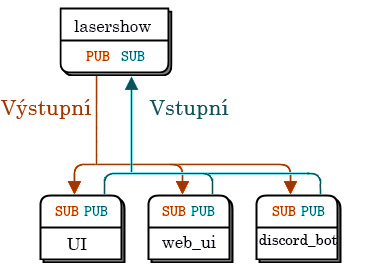
\includegraphics[width=0.9\textwidth]{img/comms_lasershow_scheme.jpg}
    \caption{\label{fig:lasershow_comms} Komunikace mezi programy vstupním socketem na~portu 5557}
  \end{minipage}\hfill
  \begin{minipage}{0.45\textwidth}
    \centering
    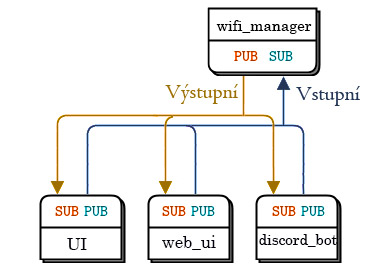
\includegraphics[width=0.9\textwidth]{img/comms_wifiman_scheme.jpg}
    \caption{\label{fig:wifiman_comms} Komunikace mezi programy výstupním socketem na~portu 5556}
  \end{minipage}
\end{figure}

Jednotlivé příkazy, které můžou prorgamy lasershow přijímat, jsou popsány v příloze v souboru README.md. Tento soubor se totiž na serveru github.com, kam byl projekt vystaven, zobrazuje přímo na domovské stránce projektu a kdokoliv, koho by projekt zajímal si je tam rychle najde.
